\documentclass{report}
\usepackage[utf8]{inputenc}

\usepackage{graphicx}
 \usepackage[]{amsthm} 
\usepackage[]{amssymb, amsmath, bm, algorithm, algorithmicx}  
\usepackage{csquotes}
\usepackage[noend]{algpseudocode}

\newtheorem{lemma}{Lemma}

\title{Distributed Coded Computation}
\author{Pedro J. Soto}
\date{March 2021}

\begin{document}

\maketitle

\begin{abstract}
A ubiquitous problem in computer science research is the optimization of computation on large data sets. Such computations are usually too large to be preformed on one machine and therefore the task needs to be distributed amongst a network of machines. However, a common problem within distributed computing is the mitigation of delays caused by faulty machines in the network or traffic congestion. This can be performed by the use of coding theory to optimize the amount of redundancy needed to handle such faults.  This problem differs from classical coding theory insofar that it is concerned with the dynamic coded computation on data rather than just statically coding data without any consideration of the algorithms to be performed on said data. Of particular interest is the operation of matrix multiplication, which happens to be a fundamental operation in many big data/machine learning algorithms, which is the main focus of this paper. Two wonderful consequences of the (bi-)linear nature of matrix multiplication is that it is both highly parrallelizable and that linear codes can be applied to it; making the coding theory approach a fruitful avenue of research for this particular optimization of distributed computing. 
\end{abstract}

\tableofcontents



\chapter{Introduction}

Due to the atomic limit, the rate at which CPU's get smaller slows and distributed computing has become a more ubiquitous and necessary topic in both research and the lives of ordinary consumers of computer technology. 
Another reason for the rise of distributed computing is that data sets have become very large and the computations performed on them must be split amongst many machines. 
In a distributed setting a large task is split up into smaller tasks that are run in parallel amongst the machines, or \textit{nodes}, in the network. 

However, it is well known that nodes in a distributed infrastructure are commonly composed of commodity hardware which are more likely to be subject to various faulty behaviors~\cite{Huang2017a}. 
One example of such a fault is when a node may experiences a temporary performance degradation due to load imbalance or resource congestion~\cite{Lee2018a}. 
In particular, the performance of virtual machines in Amazon EC2 clusters have been observed to have a performance degradation of up to a factor of $5$~\cite{Tandon2017, Lee2018a}. 
A node may even fail to complete a task due to hardware failures, network partition, or power failures. 
In a Facebook data center, it has been reported that up to more than 100 such failures can happen on a daily basis~\cite{Rashmi2013,Sathiamoorthy2013}.
% Couldn't figure out how to change this sentance.
Therefore, when the computation is distributed onto multiple nodes, its progress can be significantly affected by the tasks running on such slow or failed
nodes, which we call {\em stragglers}.

\section{Problem Formulation}

In general we have some computation $f$ that we wish to perform on some data-set $D$. If the data-set $D$ or the computation $f$ becomes too large/expensive to perform on one machine, then the computation and the data set must be split up, or \emph{partitioned}, into smaller \emph{tasks} $\mathcal{P} : f(D) \mapsto f_1(D_1) ,..., f_k(D_k)$ as illustrated in fig~\ref{fig:1}. 
\begin{figure}
    \centering
    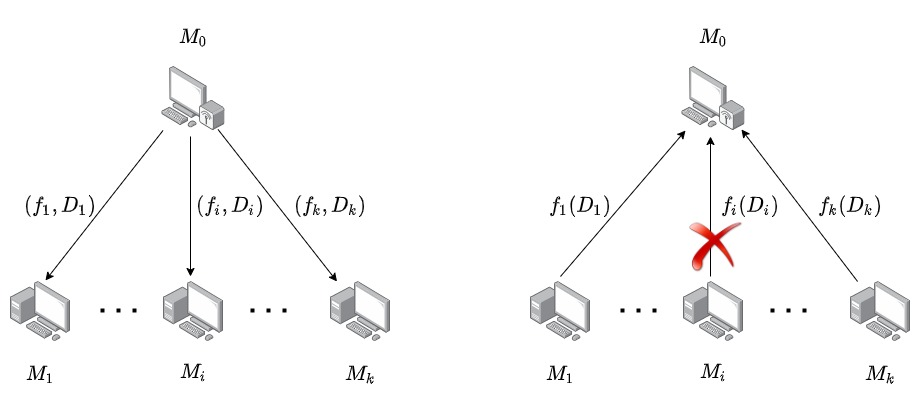
\includegraphics[width=\textwidth]{straggler_diag_1.jpg}
    \caption{The task $f(D)$ is too large to do on machine $M_0$ so it partitions the job into some smaller tasks $f_1(D_i), ..., f_k(D_k)$ and distributes it amongst the workers. Supposing that the machine $M_i$ takes a long (possibly infinite) time $t_i$ to finish then the desired computation of $f(D)$ is delayed by time $t_i$.}
    \label{fig:1}
\end{figure}
We wish to do so in a way that recreating the original job, $f(D)$ from the tasks $f_1(D_1) , ..., f_k(D_K)$ has very little overhead (\emph{i.e.,} we wish to minimize the complexity of $\mathcal{P}^{-1}$). 
In particular, if one of the machines, say $M_i$, takes a long time, say $t_i$, to compute $f_i(D_i)$ \textit{then the entire algorithm is delayed by the time $t_i$.} In the worst case, machine $M_i$ never finishes and the computation $f(D)$ is never completed. 
The main idea is to add some redundant tasks $f_{k+1}(D_{k+1}),...,f_{k+r}(D_{k+r})$ to $\mathcal{P}$ so as to mitigate the possibility of stragglers (\emph{i.e.,} so that we can recreate $f(D)$ without needing the datum $f_i(M_i)$).
However, this cannot be done naively; we will show in sec.~\ref{sec:mot_ex} that merely replicating the same tasks on other workers will not suffice since it is highly inefficient and can suffer from the same faults it is trying to solve. Therefore it becomes necessary to apply error-correcting codes, or more precisely \textit{erasure codes}, to the problem. In particular the naive partition, replication, and recreating in $\mathcal{P},\mathcal{P}^{-1}$ are replaced with \emph{encoding} and \emph{decoding} functions $\mathcal{E},\mathcal{D}$ of an erasure code (see sec.~\ref{sec:code}). 

\section{Motivating Example}\label{sec:mot_ex}

Consider the following toy example: $M_0$ wishes to compute the product of the two matrices 
\begin{equation*}
    A = \begin{bmatrix}a_{1,1} & a_{1,2} \\ 
    a_{2,1} & a_{2,2} \\ \end{bmatrix} , \     B = \begin{bmatrix}b_{1,1} & b_{1,2} \\ 
    b_{2,1} & b_{2,2} \\ \end{bmatrix}
\end{equation*}
but computing $AB$ would take too long to compute on one machine. $M_0$ could send $A_1 = \begin{bmatrix}a_{1,1} & a_{1,2} \\ \end{bmatrix} $ to $M_1$ and send $A_2 = \begin{bmatrix}a_{2,1} & a_{2,2} \\ \end{bmatrix}$ to $M_2$ and in addition send $B$ to both workers as indicated by fig.~\ref{fig:2}. 
Since it is easy to verify that 
\begin{equation}\label{eq:1}
 \begin{bmatrix}A_1B \\ 
    A_2B  \\ \end{bmatrix}=  \begin{bmatrix}A_1B \\ 
    0  \\ \end{bmatrix}   +  \begin{bmatrix}0\\ 
    A_2B\\ \end{bmatrix} =   \begin{bmatrix}a_{1,1} & a_{1,2} \\ 
    0 & 0 \\ \end{bmatrix} B  +  \begin{bmatrix}0& 0\\ 
    a_{2,1} & a_{2,2} \\ \end{bmatrix} B = AB , 
\end{equation}
a valid scheme would be to have $M_1$ compute $A_1 B$ and have $M_2$ compute $A_2 B$ and then combine the results in the obvious way implied by eq.~\eqref{eq:1} as indicated in fig.~\ref{fig:2}. 
\begin{figure}
    \centering
    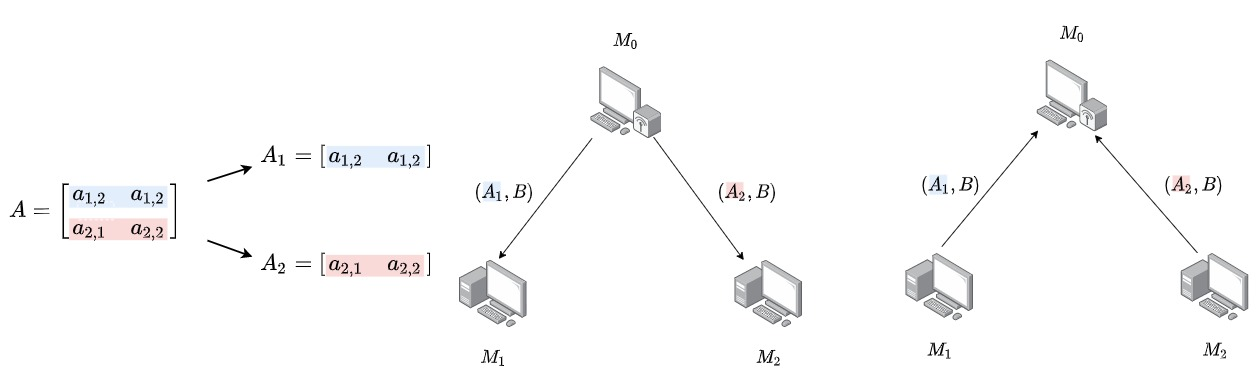
\includegraphics[width=\textwidth]{dist_diag_1.jpg}
    \caption{The master first splits $A$ into smaller sub-matrices $A_1$ and $A_2$. Then the master sends the tasks $(A_1,B)$ and $(A_2,B)$ to be multiplied by machines $M_1$ and $M_2$ respectively. As indicated by eq.~\eqref{eq:1} the master can then recreate the original job $AB$ from these two sub-tasks.}
    \label{fig:2}
\end{figure}

A naive way to mitigate the possibility of $M_1$ or $M_2$ becoming a straggler is to use \textit{replication}. For example we can replicate the tasks on two other machines $M_3,M_4$ by sending $(A_1,B)$ to $M_3$ and sending $(A_2,B)$ to $M_4$ as depicted in the first diagram of fig.~\ref{fig:3}. 
\begin{figure}
    \centering
    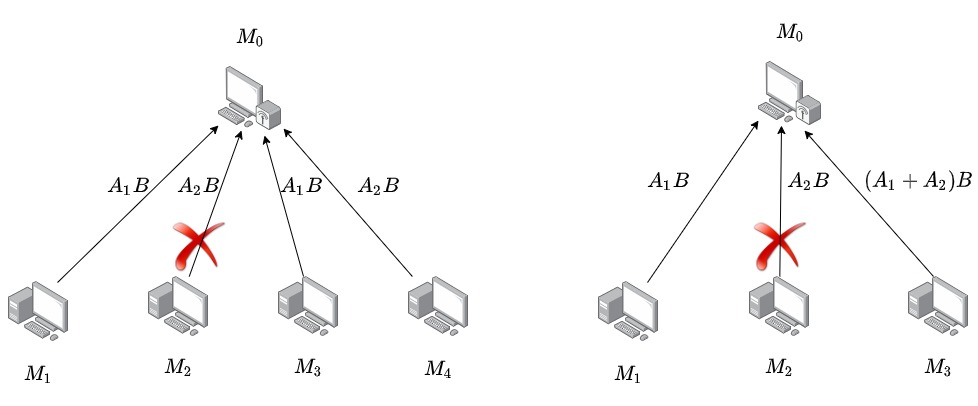
\includegraphics[width=\textwidth]{strag_diag_2.jpg}
    \caption{
    The first diagram depicts the naive ``replication coding scheme'' and the second diagram depicts the coding theory approach. The naive ``replication coding scheme'' one must use 4 machines to handle one fault whereas the erasure code only needs 3.
    }
    \label{fig:3}
\end{figure}
But a more efficient way to mitigate these stragglers is to create a ``parity'' task $(A_1+A_2)B$ and send it to $M_3$ as shown in the second diagram of fig.~\ref{fig:3}. Since matrix multiplication is linear in both of its arguments, we have that $(A_1+A_2)B = A_1B+A_2B$; therefore, if a machine, say $M_2$, becomes a straggler then $M_0$ can recreate the task by computing 
\begin{equation*}
    M_{3}^\text{result} - M_{1}^\text{result} =  (A_1+A_2)B - A_1B = A_1B+A_2B- A_1B = A_2B = M_2^\text{result}.
\end{equation*}
Like wise if $M_1$ had been the straggler one could have recreated the task by subtracting the result from machine from $M_3$ from the result from $M_2$. Thus we have given a procedure for ``encoding'' and ``decoding'' (see sec.~\ref{sec:code}) the computation so as to handle any possible failure of one of the machines $M_1$, $M_2$, or $M_3$ and more it uses 3 machines instead of 4, \emph{i.e., it uses less resources}.

However, one could argue that in a particular scenario that they have an extra machine to spare, but it is important to note that, the coding theory approach also mitigates risk with a higher probability as well when given the same amount of resources. To be more precise, one could extend the example given in fig.~\ref{fig:3} to the one given in fig.~\ref{fig:4}. 
\begin{figure}
    \centering
    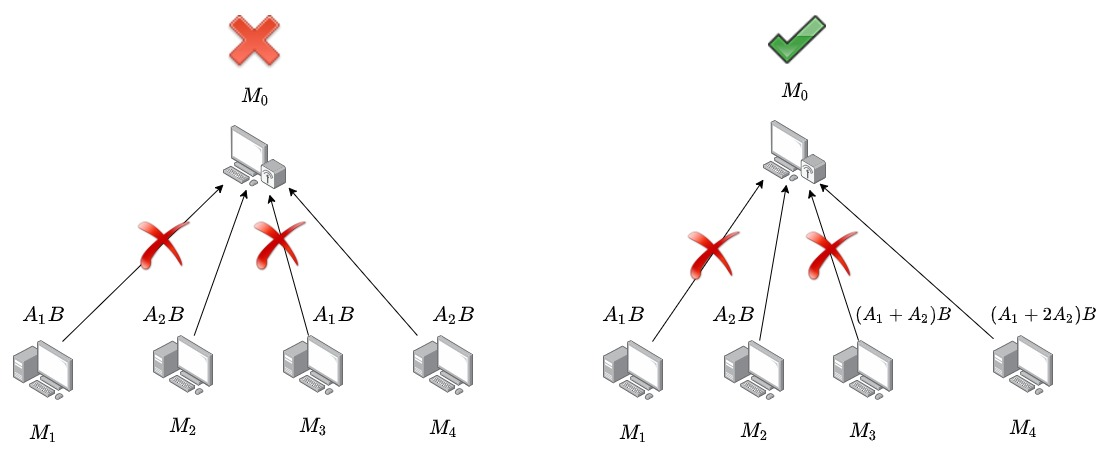
\includegraphics[width=\textwidth]{strag_diag_3.jpg}
    \caption{
    The first diagram depicts the naive ``replication coding scheme'' and the second diagram depicts the coding theory approach with the same amount of resources. The naive ``replication coding scheme'' cannot handle 2 faults in general while erasure coding can handle \textit{any} two faults.
    }
    \label{fig:4}
\end{figure}
As shown in the second diagram of fig.~\ref{fig:4} we can extend the code by adding a second parity task $(A_1+2A_2)B$ and giving it the 4 machine. \textit{The amazing thing about this procedure is that it can now handle any 2 out of 4 faults.} This is easily verified by checking that any two rows of the matrix $\mathcal{E} $ in the system of equations given by
\begin{equation}\label{eq:firstcode}
    \mathcal{E} \begin{bmatrix}
       A_1 B\\ A_2B \\ 
    \end{bmatrix} =  \begin{bmatrix}
       1 & 0 \\
       0& 1\\ 
       1 &1 \\
       1 & 2\\
    \end{bmatrix} \begin{bmatrix}
       A_1 B\\ A_2B \\ 
    \end{bmatrix} =  \begin{bmatrix}
       M_1^\text{result}\\
       M_2^\text{result}\\ 
       M_3^\text{result} \\
       M_4^\text{result}\\
    \end{bmatrix} 
\end{equation}
are linearly independent (see sec.~\ref{sec:lin}) and thus given any two $M^\text{result}_i$ allows us to solve the linear system solve for the values of $A_1B,A_2B$. For example in the case given in the second diagram of fig.~\ref{fig:4} we can recreate $M_1$ by computing $M_{4}^\text{result} - 2M_{2}^\text{result} = A_1B = M_1^\text{result}$. In particular, we have that $M_1$ and $M_3$ failing correspond to deleting the first and second rows of the $\mathcal{E}$ in eq.~\eqref{eq:firstcode} and since rows 2 and 4 of $\mathcal{E}$ are linearly independent we can solve for $A_1B,A_2B$, \emph{i.e.,} we have that 
\begin{equation*}
    M_1, M_2 \text{ fail } \implies 
\end{equation*}\begin{equation}\label{eq:firstcode}
    \mathcal{E}_\text{fail} \begin{bmatrix}
       A_1 B\\ A_2B \\ 
    \end{bmatrix} =  \begin{bmatrix}
       0& 1\\ 
       1 & 2\\
    \end{bmatrix} \begin{bmatrix}
       A_1 B\\ A_2B \\ 
    \end{bmatrix} =  \begin{bmatrix}
       M_2^\text{result}\\ 
       M_4^\text{result}\\
    \end{bmatrix} 
\end{equation}
and we can solve for the desired result. \textit{However the replication code cannot survive such a fault.} As we see in the first diagram of fig.~\ref{fig:4} The information desired is lost since we have no way of retrieving the necessary $A_2B$. 


\section{Outline of the Survey}

\chapter{Background}

\section{Distributed Systems}

\section{Coding Theory}\label{sec:code}


\section{Linear Algebra and Learning Algorithms}\label{sec:lin}



\chapter{Variations of the Main Problem ({and Their Proposed Solutions})}

\section{One Large Matrix Multiplication}

\section{Multiple (\emph{i.e., Batch}) Matrix Multiplications}

\section{Partial Results/Partial Stragglers}

\section{More Complicated Functions/Machine Learning Applications}





\chapter{Our Work}

\section{Dual Entangled}

\section{Spinner}

\section{Rook Poly}

\chapter{Future Work}

\bibliographystyle{alpha}
\bibliography{references}

\end{document}
